% \section{Ablation Study: Scalability and Parallel Synthesis}
% \label{sec:ablation}

% A key architectural advantage of \methodname{} is its ability to decouple the synthesis process, which permits the parallel execution of structural planning and atomic model implementation. Predicated on the standard modeling practice where a coupled model aggregates at least two subcomponents (i.e., a branching factor $b \ge 2$), the depth of the system hierarchy grows logarithmically with the total number of components $N$. Consequently, the theoretical synthesis latency is governed by the critical path of this hierarchy rather than the sequential accumulation of all tasks. This structural property reduces the time complexity from linear $O(N)$ (characteristic of serial approaches), to logarithmic $O(\log N)$.

% To validate this, we conducted an ablation study using GPT-5.2 on the \methodname{} framework, comparing the wall-clock time of Serial execution versus Parallel execution. As shown in Figure~\ref{fig:parallel_ablation}, we analyze the speed-up across the two Stages:

% \begin{figure}[h]
%     \centering
%     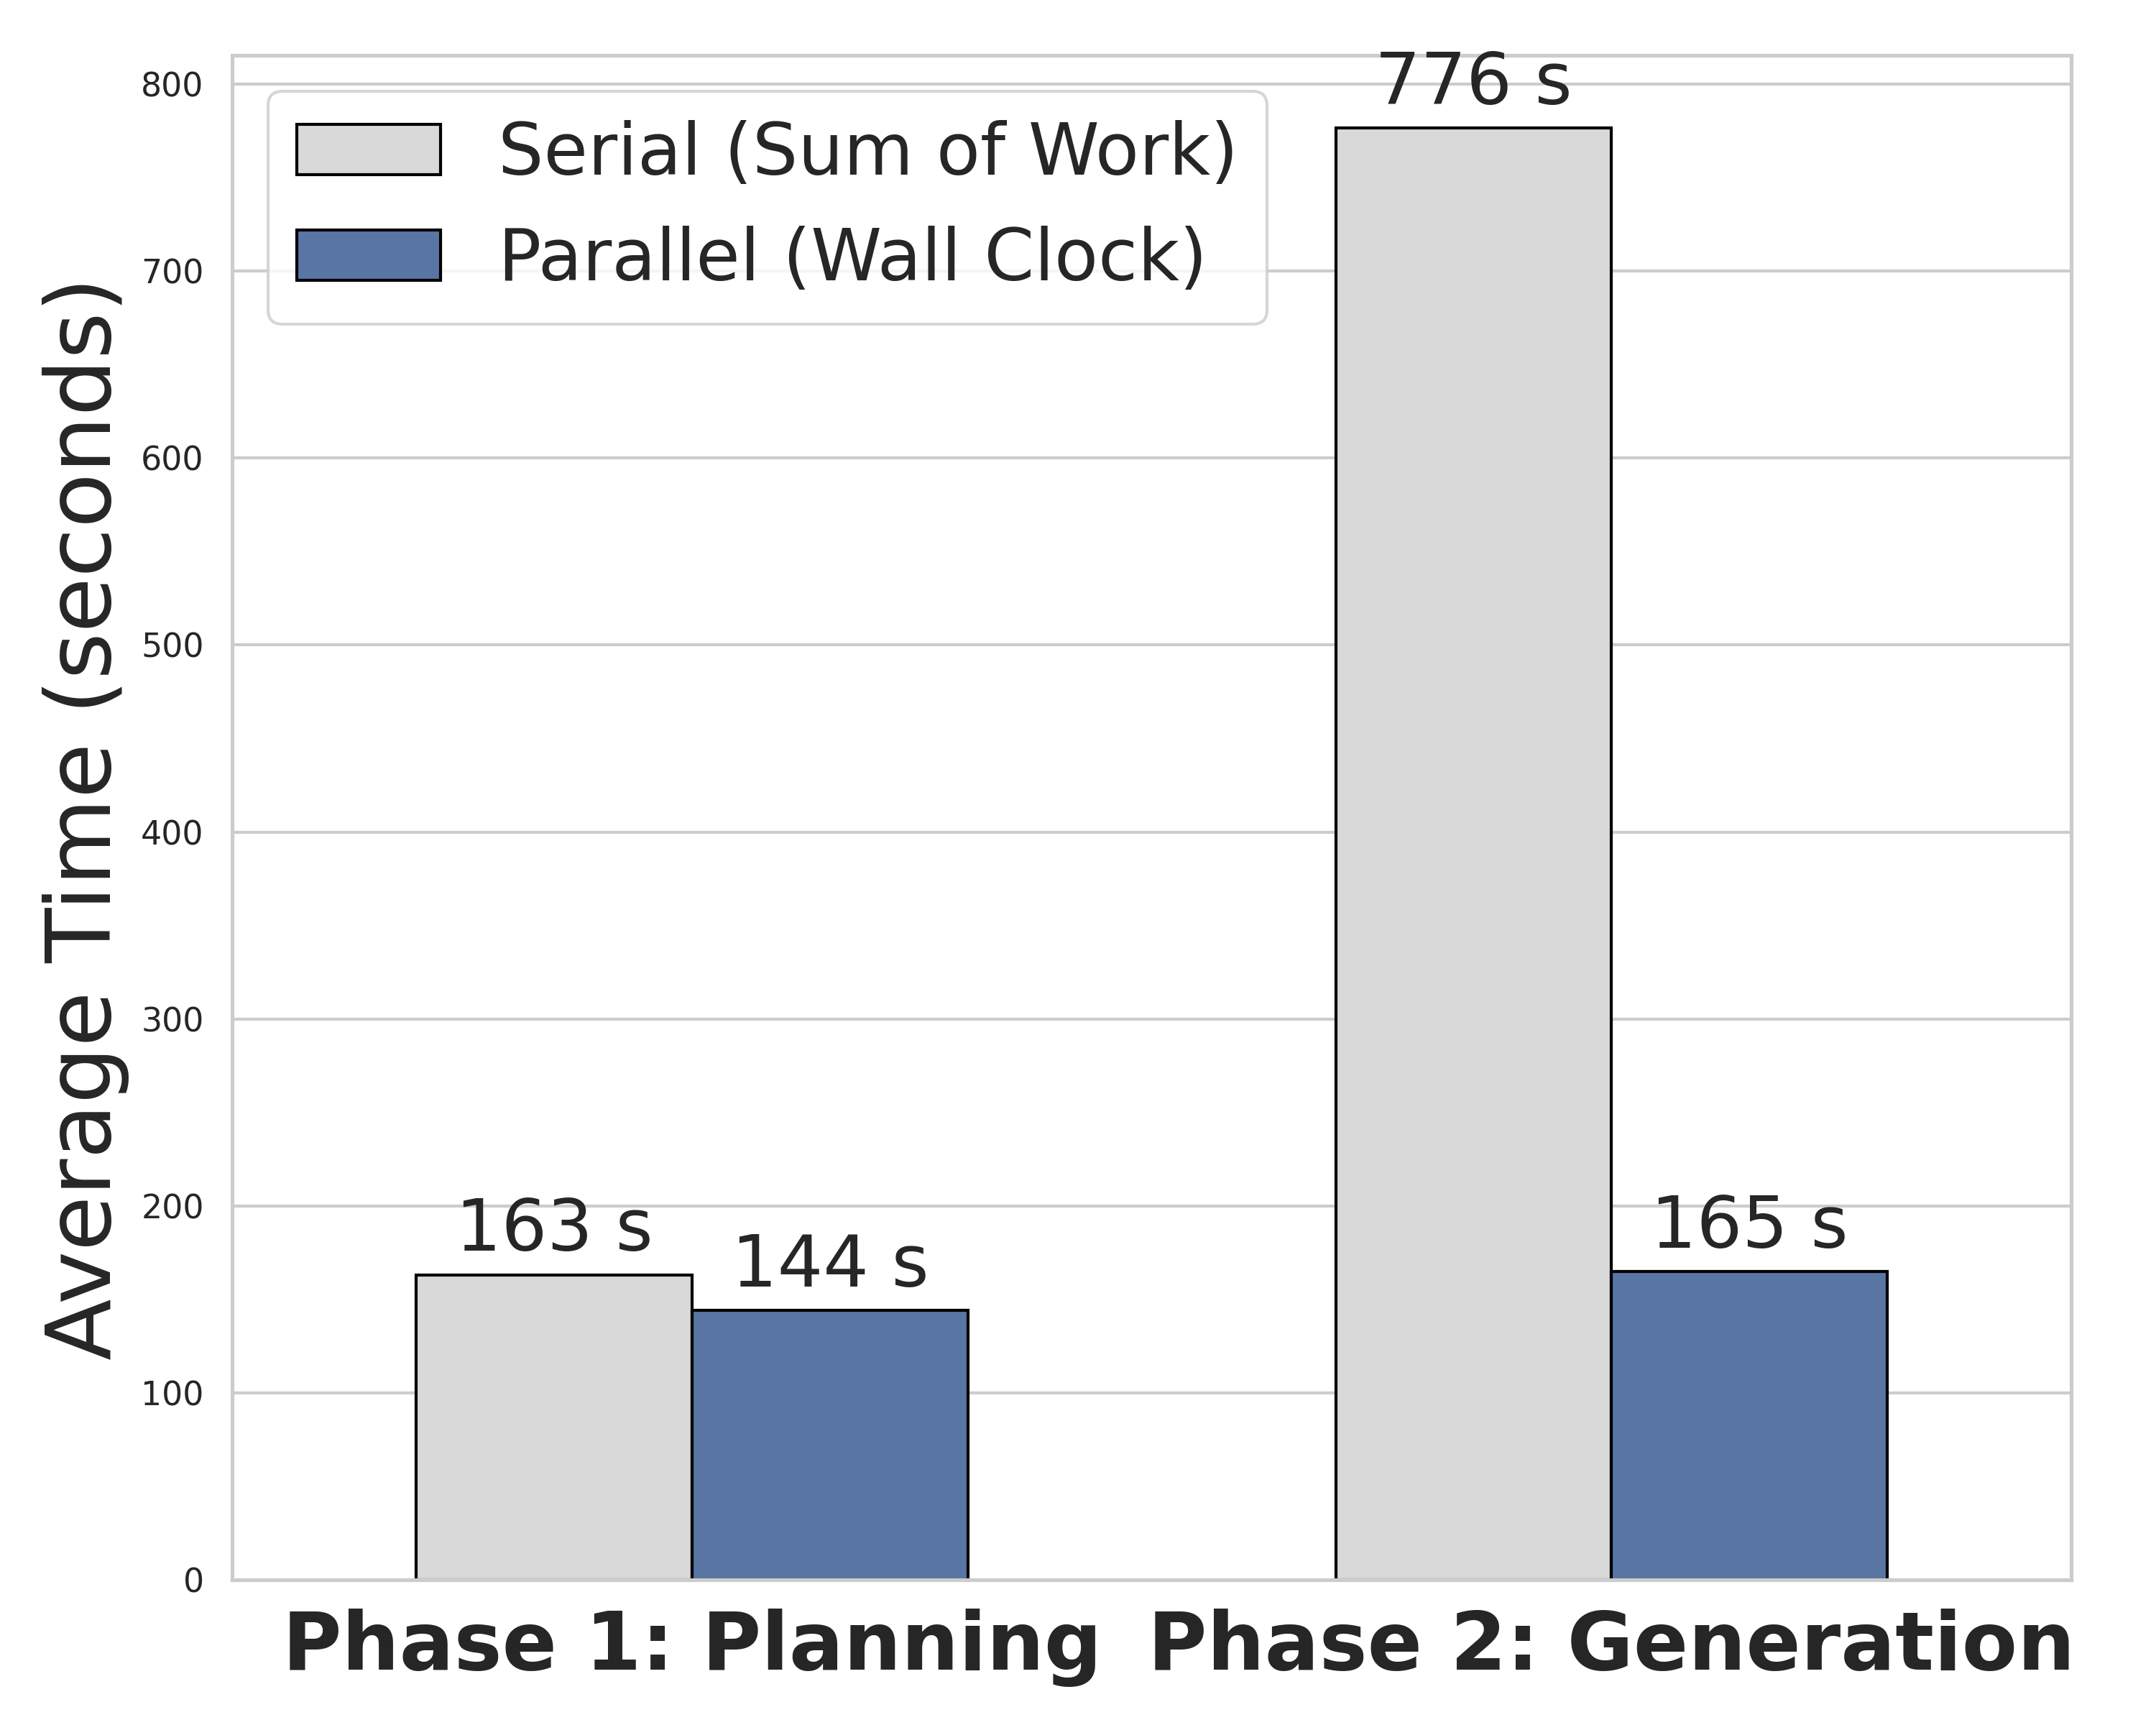
\includegraphics[width=0.5\columnwidth]{imgs/ablation_parall.png}
%     \caption{Ablation study on synthesis latency (using GPT-5.2). The chart compares the wall-clock time required for the Planning and Generation phases under serial and parallel execution modes. While the acceleration in the Planning phase is limited by the current benchmark scale, the Generation phase achieves a $4.7\times$ speedup, validating the scalability of the approach.}
%     \label{fig:parallel_ablation}
% \end{figure}

% \begin{itemize}[leftmargin=*]
%     \item \emph{Structural Planning Stage:} Theoretically, the recursive planning algorithm allows independent branches of the system hierarchy to be decomposed concurrently. However, as observed in Figure~\ref{fig:parallel_ablation}, the empirical speedup is modest. This is primarily due to the scale of our current benchmark scenarios: the system hierarchies are relatively shallow, meaning the overhead of network requests and thread management outweighs the benefits of parallelizing the lightweight component classification tasks. We expect this speedup to become significant only in much larger, deeply nested systems.
    
%     \item \emph{Behavioral Synthesizing Stage:} The acceleration is substantial, achieving a $\sim 4.7\times$ speedup. Since atomic models (leaf nodes) encapsulate the bulk of the complex logic (state transitions and logic implementation), their generation is the computational bottleneck. Our framework successfully isolates these tasks, allowing them to be synthesized simultaneously. 
% \end{itemize}

% This result proves the scalability of \methodname. While standard agentic loops face super-linear growth in time and context costs as system complexity increases, our modular approach ensures that the synthesis time grows logarithmically, making it feasible for large-scale world modeling.